
Neste capítulo, serão descritos os conjuntos de dados utilizados neste trabalho, bem como os processos de extração e transformação envolvidos.

\section{Dados de Documentos Fiscais}
\label{section:dados-de-documentos-fiscais}

Nesta seção, será apresentado o tratamento dos dados obtidos através da coleta de documentos fiscais.

\subsection{Aquisição}

Como descrito na Seção~\ref{section:arquivei}, os dados utilizados neste trabalho são obtidos através do armazém de dados da empresa parceira. Estes dados passam por um complexo processo de ingestão e tratamento descrito em detalhes no Apêndice~\ref{chapter:armazem-de-dados}.

A seleção dos dados foi feita usando o armazém de dados, através da linguagem \sigla{SQL}{\textit{Structured Query Language}}. Os critérios de seleção utilizados para obter os dados do armazém de dados foram:

\begin{itemize}
    \item Foram utilizados apenas dados de Notas Fiscais Eletrônicas, excluindo outros documentos fiscais
    \item Foram utilizados apenas documentos obtidos através do \textit{webservice} da Sefaz
    \item Foram utilizados apenas dados de documentos emitidos entre 01 de janeiro de 2019 e 31 de outubro de 2020
    \item Foram utilizados apenas documentos contendo a assinatura digital do emitente
    \item Foram utilizados apenas documentos contendo o protocolo de processamento do \textit{webservice} da Sefaz
    \item Foram utilizados apenas documentos cuja emissão foi autorizada pelo \textit{webservice} da Sefaz
    \item Foram utilizados apenas documentos referentes a transações cujo \sigla{CFOP}{Código Fiscal de Operações e Prestações} se refere às movimentações entre empresas envolvendo comercialização de mercadorias. Esses critérios são explicados em detalhes no Apêndice~\ref{chapter:cfop}
\end{itemize}

Os campos considerados são descritos no Quadro~\ref{quadro:campos-considerados-nfe}. Os tipos de dados e suas peculiaridades são descritos no Apêndice~\ref{chapter:tecnologias-utilizadas}.

\begin{quadro}[htb]
\caption{Campos de documentos fiscais considerados}
\label{quadro:campos-considerados-nfe}
\centering
\begin{tabular}{|l|l|l|}        \hline
\textbf{Nome do campo} & \textbf{Tipo de dado} & \textbf{Descrição}            \\ \hline
ID               & STRING       & Chave de acesso da NFe (anonimizado)         \\ \hline
dhEmi            & DATETIME     & Data e Hora de emissão do Documento Fiscal   \\ \hline
emit             & RECORD       & Identificação do Destinatário                \\
emit.CNPJ        & STRING       & Número do CNPJ do emitente (anonimizado)     \\ \hline
dest             & RECORD       & Identificação do Destinatário                \\
dest.CNPJ        & STRING       & Número do CNPJ do destinatário (anonimizado) \\ \hline
det              & ARRAY        & Dados dos detalhes da NF-e                   \\
det.prod         & RECORD       & Dados dos produtos e serviços da NF-e        \\
det.prod.\_nItem & INTEGER      & Número do item do NF                         \\
det.prod.VProd   & FLOAT        & Valor bruto do produto ou serviço            \\
det.prod.CFOP    & STRING       & CFOP                                         \\ \hline
\end{tabular}
\end{quadro}

Cada linha do conjunto de dados possui dados de uma transação entre duas empresas, identificada por uma chave de acesso única por transação, e que contém um ou mais produtos envolvidos com seus respectivos números de item, valor bruto, e CFOP.

Todos os dados obtidos a partir do armazém de dados foram anonimizados. Dados identificadores ou sensíveis foram removidos e reindexados de forma a manter o sigilo e privacidade de tais dados respeitando tanto a legislação atual quanto os contratos de prestação de serviços da empresa parceira.

\subsection{Pré-processamento}

Para cada documento foi criada uma nova coluna com o valor bruto agregado dos produtos transacionados, respeitando os critérios de CFOP e sendo eliminados os documentos de valor zero (o que é possível devido a inconsistências durante a emissão do documento).

Para remover eventuais problemas de completude nos dados, foram considerados apenas documentos de transações entre empresas recorrentes. Chamamos de \textbf{empresas recorrentes} aquelas que possuem pelo menos um documento na base de dados emitido para cada mês entre janeiro de 2019 e outubro de 2020.

Uma vez tratados os dados, estes foram agregados em três conjuntos adicionais de dados, agregados por:

\begin{itemize}
    \item \sigla{UF}{Unidade Federativa}
    \item Seção de CNAE
    \item CNAE
\end{itemize}

Cada um dos três conjuntos de dados agrega informações das transações efetuadas durante um mês, de janeiro de 2019 a outubro de 2020, sendo agregada a informação do valor total bruto dos produtos transacionados.

Uma nova coluna foi criada contendo a quantidade de transações mensal entre cada entidade. Foi considerado que cada NF-e documenta uma única transação independente da quantidade de produtos envolvida.

\section{Dados Abertos de Empresas Brasileiras}
\label{section:dados-abertos-receita}

Nesta seção, será apresentado o tratamento dos dados obtidos através da base de dados abertos da Receita Federal.

\subsection{Aquisição}

Além dos dados descritos na Seção~\ref{section:dados-de-documentos-fiscais}, foram utilizados também dados coletados das bases de dados abertas sobre o Cadastro Nacional de Pessoas Jurídicas da Receita Federal \cite{receita:dados-publicos:cnpj}.

Tais dados são divulgados conforme previsto no Artigo 5º da Constituição Federal \cite{constituicao:1988}:

\begin{citacao}
Art. 5º Todos são iguais perante a lei, sem distinção de qualquer natureza, garantindo-se aos brasileiros e aos estrangeiros residentes no País a inviolabilidade do direito à vida, à liberdade, à igualdade, à segurança e à propriedade, nos termos seguintes:

...

XXXIII - todos têm direito a receber dos órgãos públicos informações de seu interesse particular, ou de interesse coletivo ou geral, que serão prestadas no prazo da lei, sob pena de responsabilidade, ressalvadas aquelas cujo sigilo seja imprescindível à segurança da sociedade e do Estado;

...
\end{citacao}

Regulado pela Lei de Acesso a Informação \cite{lei:12527:lei-de-acesso-a-informacao}:

\begin{citacao}
Art. 8º É dever dos órgãos e entidades públicas promover, independentemente de requerimentos, a divulgação em local de fácil acesso, no âmbito de suas competências, de informações de interesse coletivo ou geral por eles produzidas ou custodiadas.

...

§ 3º Os sítios de que trata o § 2º deverão, na forma de regulamento, atender, entre outros, aos seguintes requisitos:

...

III - possibilitar o acesso automatizado por sistemas externos em formatos abertos, estruturados e legíveis por máquina;

...
\end{citacao}

Esses dados são também tratados e estão disponíveis no armazém de dados da empresa parceira através do processo descrito no Apêndice~\ref{chapter:armazem-de-dados}. De lá foram coletadas as seguintes informações a partir da base de dados completa, cujos campos são descritos no Quadro~\ref{quadro:campos-considerados-nfe}.

\begin{quadro}[htb]
\caption{Campos do Cadastro Nacional de Pessoas Jurídicas considerados}
\label{quadro:campos-considerados-cnpj}
\centering
\begin{tabularx}{\textwidth}{|l|l|X|} \hline
\textbf{Nome do campo} & \textbf{Tipo de dado} & \textbf{Descrição}                   \\ \hline
CNPJ                & STRING       & Número de Inscrição no CNPJ                      \\ \hline
SituacaoCadastral   & STRING       & Código da Situação Cadastral                     \\ \hline
DataInicioAtividade & STRING       & Data de Início da Atividade                      \\ \hline
CnaeFiscal          & STRING       & Código da Atividade Econômica                    \\ \hline
UF                  & STRING       & Sigla da UF em que se encontra o estabelecimento \\ \hline
Municipio           & STRING       & Código do município de jurisdição onde se encontra o estabelecimento \\ \hline
Porte               & STRING       & Código do porte da empresa                       \\ \hline
OpcaoSimples        & STRING       & Indicador da existência da opção pelo simples    \\ \hline
OpcaoMei            & STRING       & Indicador da existência da opção pelo MEI        \\ \hline
\end{tabularx}
\end{quadro}

Através do número de inscrição das empresas foi possível cruzar os dados obtidos nesta base de dados com a base de dados descrita na Seção~\ref{section:dados-de-documentos-fiscais}, o que foi feito antes de todo o processo de anonimização citado nessa seção.

\section{Análise Descritiva da Base de Dados}

Nesta seção, será apresentada uma análise descritiva dos dados utilizados neste trabalho, descrevendo os dados coletados de documentos fiscais e comparando sua abrangência com os dados obtidos da base de dados aberta da Receita Federal.

\subsection{Abrangência territorial}

Nesta subseção, será apresentada a análise descritiva do ponto de vista territorial. Será descrita a participação das empresas citadas na base de dados em relação aos totais de cada divisão territorial brasileira a partir dos dados descritos na Seção~\ref{section:dados-abertos-receita}.

O \sigla{IBGE}{Instituto Brasileiro de Geografia e Estatística} criou a \sigla{DTB}{Divisão Territorial Brasileira}, uma codificação hierárquica de sete dígitos do território brasileiro onde:

\begin{itemize}
    \item O primeiro dígito indica a região
    \item O segundo dígito indica a UF
    \item O terceiro e quarto dígito indicam a mesorregião
    \item O sexto dígito indica a microrregião
    \item O sétimo dígito indica o município
\end{itemize}

O Quadro~\ref{quadro:tabela-codigo-regiao} descreve as regiões brasileiras segundo esta divisão, que foi usada no estudo de abrangência territorial dos dados.

\begin{quadro}[htb]
\caption{Códigos de Região segundo DTB}
\label{quadro:tabela-codigo-regiao}
\centering
\begin{tabular}{|l|l|l|}        \hline
\textbf{Código da Região} & \textbf{Região} & \textbf{Unidade Federativa } \\ \hline
\multirow{7}{*}{1} & \multirow{7}{*}{Região Norte}        & Acre\\
  &                                      & Amapá\\
  &                                      & Amazonas\\
  &                                      & Pará\\
  &                                      & Rondônia\\
  &                                      & Roraima\\
  &                                      & Tocantins\\ \hline
\multirow{9}{*}{2} & \multirow{9}{*}{Região Nordeste}     & Alagoas\\
  &                                      & Bahia\\
  &                                      & Ceará\\
  &                                      & Maranhão\\
  &                                      & Paraíba\\
  &                                      & Pernambuco\\
  &                                      & Piauí\\
  &                                      & Rio Grande do Norte\\
  &                                      & Sergipe\\\hline
\multirow{4}{*}{3} & \multirow{4}{*}{Região Centro-Oeste} & Distrito Federal\\
  &                                      & Goiás\\
  &                                      & Mato Grosso\\
  &                                      & Mato Grosso do Sul\\ \hline
\multirow{4}{*}{4} & \multirow{4}{*}{Região Sudeste}      & Espírito Santo\\
  &                                      & Minas Gerais\\
  &                                      & São Paulo\\
  &                                      & Rio de Janeiro\\ \hline
\multirow{3}{*}{5} & \multirow{3}{*}{Região Sul}          & Paraná\\
  &                                      & Rio Grande do Sul\\
  &                                      & Santa Catarina\\ \hline
\end{tabular}
\end{quadro}

Na Figura~\ref{fig:base-de-dados:descritiva-1.1-presenca-por-regiao-1.1} é descrito o percentual do total das empresas de cada região que foi encontrada na base de dados deste trabalho. Os dados são descritos em detalhe na Tabela~\ref{tab:participacao-por-regiao}. A Figura~\ref{fig:base-de-dados:descritiva-1.2-qtde-por-regiao} descreve as quantidades de empresas presentes na base de dados em relação ao total de cada região brasileira.

Com esses dados é possível observar que a participação em termos regionais é significativa e que há um razoável balanceamento regional, com uma participação regional que varia entre 7 e 10\%, mas sem um grande viés para uma das regiões. A quantidade de empresas da Região 4 é significativamente maior em comparação à outras regiões, mas reflete proporcionalmente a realidade se verificarmos os valores percentuais.

\begin{figure}[htb]
    \centering
    \caption{Participação por região das empresas presentes na base de dados}
    \label{fig:base-de-dados:descritiva-1-presenca-por-regiao} 
    \begin{subfigure}[b]{0.45\textwidth} 
        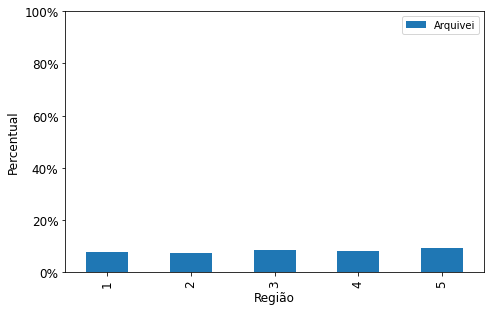
\includegraphics[scale=0.45]{images/base-de-dados-1.1-presenca-por-regiao.png}
        \caption{Percentual das empresas de cada região brasileira presente na base de dados}
        \label{fig:base-de-dados:descritiva-1.1-presenca-por-regiao-1.1}
    \end{subfigure} ~ \quad
    \begin{subfigure}[b]{0.45\textwidth}
        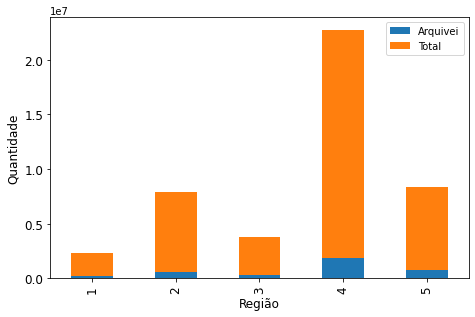
\includegraphics[scale=0.45]{images/base-de-dados-1.2-qtde-por-regiao.png}
        \caption{Quantidade de empresas de cada região brasileira presente na base de dados relativa ao total}
        \label{fig:base-de-dados:descritiva-1.2-qtde-por-regiao}
    \end{subfigure}
    \fdadospesquisa
\end{figure}

\begin{table}[htb]
\centering
\caption{Percentual das empresas presentes na base de dados por Região}
\label{tab:participacao-por-regiao}
\begin{tabular}{lr}
\toprule
Região & Participação \\
\midrule
1      &    7.88\% \\
2      &    7.26\% \\
3      &    8.41\% \\
4      &    8.00\% \\
5      &    9.39\% \\
\bottomrule
\end{tabular}
\fdadospesquisa
\end{table}

A seguir, repetimos a análise agora para as Unidades Federativas do Brasil, ilustrada em participação percentual na Figura~\ref{fig:base-de-dados:descritiva-2.1-presenca-por-uf} e na Tabela~\ref{tab:participacao-por-uf}, e em quantidades em relação à quantidade total de cada UF na Figura~\ref{fig:base-de-dados:descritiva-2.2-qtde-por-uf}.

\begin{figure}[htb]
    \centering
    \caption{Participação por UF das empresas presentes na base de dados}
    \label{fig:base-de-dados:descritiva-2-presenca-por-uf}
    \begin{subfigure}[b]{1.00\textwidth} 
        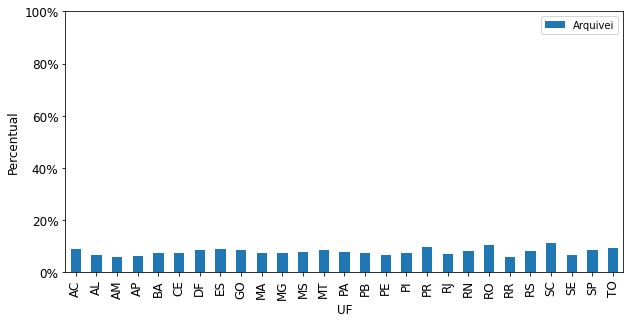
\includegraphics[scale=0.7]{images/base-de-dados-2.1-presenca-por-uf.png}
        \caption{Percentual das empresas das cada UF presente na base de dados}
        \label{fig:base-de-dados:descritiva-2.1-presenca-por-uf}
    \end{subfigure} ~ \\
    \begin{subfigure}[b]{1.00\textwidth}
        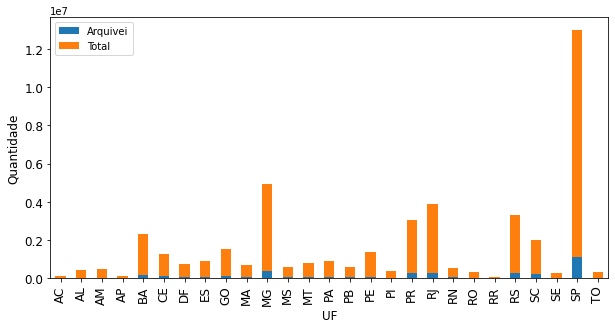
\includegraphics[scale=0.7]{images/base-de-dados-2.2-qtde-por-uf.png}
        \caption{Quantidade de empresas de cada UF presente na base de dados relativa ao total}
        \label{fig:base-de-dados:descritiva-2.2-qtde-por-uf}
    \end{subfigure}
    \fdadospesquisa
\end{figure}

\begin{table}[htb]
\centering
\caption{Percentual das empresas presentes na base de dados por UF}
\label{tab:participacao-por-uf}
\begin{subtable}[h]{0.45\textwidth}
    \centering
    \begin{tabular}{l|r}
        \toprule
        UF & Participação \\
        \midrule
        AC &    8.93\% \\
        AL &    6.75\% \\
        AM &    5.76\% \\
        AP &    6.25\% \\
        BA &    7.34\% \\
        CE &    7.46\% \\
        DF &    8.48\% \\
        ES &    8.95\% \\
        GO &    8.64\% \\
        MA &    7.56\% \\
        MG &    7.41\% \\
        MS &    7.67\% \\
        MT &    8.44\% \\
        PA &    7.91\% \\
        \bottomrule
    \end{tabular}
\end{subtable}
\begin{subtable}[h]{0.45\textwidth}
    \centering
    \begin{tabular}{l|r}
        \toprule
        UF & Participação \\
        \midrule
        PB &    7.43\% \\
        PE &    6.68\% \\
        PI &    7.49\% \\
        PR &    9.58\% \\
        RJ &    7.14\% \\
        RN &    8.03\% \\
        RO &    0.34\% \\
        RR &    6.04\% \\
        RS &    8.16\% \\
        SC &    1.15\% \\
        SE &    6.45\% \\
        SP &    8.41\% \\
        TO &    9.13\% \\
        \bottomrule
    \end{tabular}
\end{subtable}
\fdadospesquisa
\end{table}

Da mesma forma, é possível observar que a participação por unidade federativa é significativa e que embora haja um desbalanceamento um pouco maior, com uma participação por UF que varia entre 6 e 12\%, também não há um grande viés percentual para uma das UFs, refletindo razoavelmente a realidade.

Por fim, a Figura~\ref{fig:base-de-dados:descritiva-3.1-presenca-por-mun} mostra um histograma relacionando o percentual do total de empresas presentes na base de dados em relação aos municípios brasileiros. A Tabela~\ref{tab:participacao-por-mun} mostra algumas métricas sobre esta análise por municípios, mostrando que existe participação em todos os municípios brasileiros com uma média e mediana próximos de 7.5\% e pico de 21\%.

\begin{figure}[htb]
    \centering
    \caption{Histograma do percentual das empresas de cada município brasileiro presente na base de dados}
    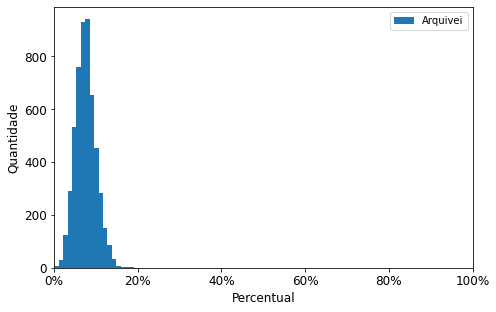
\includegraphics[scale=0.7]{images/base-de-dados-3.1-presenca-por-mun.png}
    \label{fig:base-de-dados:descritiva-3.1-presenca-por-mun}
    \fdadospesquisa
\end{figure}

\begin{table}[htb]
\centering
\caption{Métricas sobre o percentual das empresas presentes na base de dados por município}
\label{tab:participacao-por-mun}
\begin{tabular}{lr}
\toprule
Métrica & Valor \\
\midrule
Média         &    7.522\% \\
Desvio Padrão &    2.462\% \\
Mínimo        &    0.002\% \\
25º percentil &    5.834\% \\
50º percentil &    7.419\% \\
75º percentil &    9.065\% \\
Máximo        &   21.230\% \\
\bottomrule
\end{tabular}
\fdadospesquisa
\end{table}

Assim, pode-se observar uma forte participação territorial dos dados tanto observando do ponto de vista regional como também estadual e municipal, estando presentes nas mais diversas realidades brasileiras.

\subsection{Abrangência econômica}

Os dados descritos na Seção~\ref{section:dados-abertos-receita} apresentam uma série de informações e classificações das empresas que podem ser utilizadas para ter uma melhor noção do porte e dos tipos de empresas envolvidas. Nesta subseção, será apresentada a análise descritiva do ponto de vista econômico em relação aos totais coletados daquela base.

A primeira classificação que vamos considerar para esta análise é o \textbf{porte} de uma empresa. Regulada pela Lei nº 5172/1966 ~\cite{lei:5172:codigo-tributario}, que em seu Artigo 3º define:

\begin{citacao}
Art. 3º Para os efeitos desta Lei Complementar, consideram-se \textbf{microempresas} ou \textbf{empresas de pequeno porte}, a sociedade empresária, a sociedade simples, a empresa individual de responsabilidade limitada e o empresário a que se refere o art. 966 da Lei no 10.406, de 10 de janeiro de 2002 (Código Civil), devidamente registrados no Registro de Empresas Mercantis ou no Registro Civil de Pessoas Jurídicas, conforme o caso, desde que:

I - no caso da microempresa, aufira, em cada ano-calendário, receita bruta igual ou inferior a R\$ 360.000,00 (trezentos e sessenta mil reais); e

II - no caso de empresa de pequeno porte, aufira, em cada ano-calendário, receita bruta superior a R\$ 360.000,00 (trezentos e sessenta mil reais) e igual ou inferior a R\$ 4.800.000,00 (quatro milhões e oitocentos mil reais).

§ 1º  Considera-se receita bruta, para fins do disposto no caput deste artigo, o produto da venda de bens e serviços nas operações de conta própria, o preço dos serviços prestados e o resultado nas operações em conta alheia, não incluídas as vendas canceladas e os descontos incondicionais concedidos.

(...)
\end{citacao}

As empresas declaram seu porte no momento da sua inscrição no Cadastro Nacional de Pessoas Jurídicas, e esta declaração é revisada pela Receita Federal a partir de suas declarações fiscais anuais. Empresas cuja receita bruta não se enquadra nas categorias \sigla{ME}{Microempresa} e \sigla{EPP}{Empresa de Pequeno Porte} são enquadradas na categoria \textbf{Demais}. Em alguns casos específicos, as empresas não declaram sua receita bruta no ato da inscrição no cadastro, em sua maioria empresas estrangeiras presentes no cadastro, essas são enquadradas na categoria \textbf{Não Informado}.

A partir dos dados das Figuras~\ref{fig:base-de-dados:descritiva-4.1-presenca-por-porte} e~\ref{fig:base-de-dados:descritiva-4.2-qtde-por-porte} é possível verificar a participação das empresas presentes na base de dados em relação aos totais. A Tabela~\ref{tab:participacao-por-porte} descreve os valores em detalhes.

\begin{figure}[htb]
    \centering
    \caption{Participação por porte das empresas presentes na base de dados}
    \label{fig:base-de-dados:descritiva-4-presenca-por-porte}
    \begin{subfigure}[b]{0.45\textwidth} 
        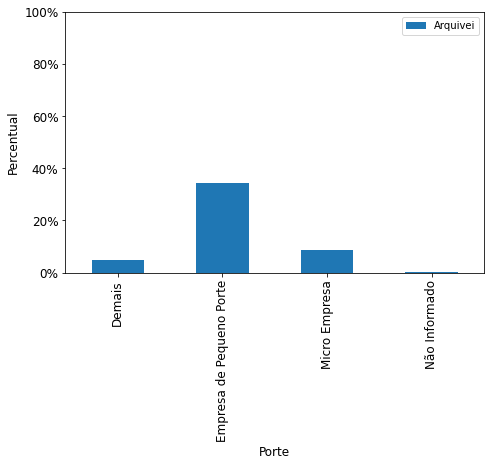
\includegraphics[scale=0.45]{images/base-de-dados-4.1-presenca-por-porte.png}
        \caption{Percentual das empresas presente na base de dados categorizadas por porte}
        \label{fig:base-de-dados:descritiva-4.1-presenca-por-porte}
    \end{subfigure} ~ \quad
    \begin{subfigure}[b]{0.45\textwidth}
        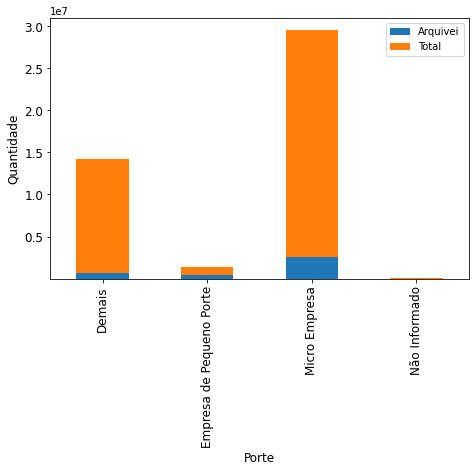
\includegraphics[scale=0.45]{images/base-de-dados-4.2-qtde-por-porte.png}
        \caption{Quantidade de empresas categorizadas por porte presente na base de dados relativa ao total}
        \label{fig:base-de-dados:descritiva-4.2-qtde-por-porte}
    \end{subfigure}
    \fdadospesquisa
\end{figure}

\begin{table}[htb]
\centering
\caption{Métricas sobre o percentual das empresas presentes na base de dados por porte}
\label{tab:participacao-por-porte}
\begin{tabular}{lr}
\toprule
Porte & Participação \\
\midrule
Demais                   &    4.76\% \\
Empresa de Pequeno Porte &    34.46\% \\
Micro Empresa            &    8.59\% \\
Não Informado            &    0.05\% \\
\bottomrule
\end{tabular}
\fdadospesquisa
\end{table}

É possível observar que há uma participação significativa desproporcional maior de EPPs nas empresas presentes da base de dados em relação à base de comparação. A participação é significativa também nos segmentos de Micro Empresas e Demais. Dentre as empresas que não informaram o porte a participação é proporcionalmente bastante baixa e suas quantidades totais na base de comparação são também muito pequenas.

A legislação brasileira define também a figura do \sigla{MEI}{Microempreendedor Individual} através do Código Civil Brasileiro \cite{lei:10406:lei-codigo-civil} que define a figura do empresário como:

\begin{citacao}
Art. 966. Considera-se empresário quem exerce profissionalmente atividade econômica organizada para a produção ou a circulação de bens ou de serviços.

Parágrafo único. Não se considera empresário quem exerce profissão intelectual, de natureza científica, literária ou artística, ainda com o concurso de auxiliares ou colaboradores, salvo se o exercício da profissão constituir elemento de empresa.
\end{citacao}

E da Lei nº 128/2008 \cite{lei:128:lei-mei} que estende essa definição para a figura do MEI:

\begin{citacao}
Art. 18-A.  O \textbf{Microempreendedor Individual - MEI} poderá optar pelo recolhimento dos impostos e contribuições abrangidos pelo Simples Nacional em valores fixos mensais, independentemente da receita bruta por ele auferida no mês, na forma prevista neste artigo.

§ 1o  Para os efeitos desta Lei, considera-se MEI o empresário individual a que se refere o art. 966 da Lei no 10.406, de 10 de janeiro de 2002 – Código Civil, que tenha auferido receita bruta, no ano-calendário anterior, de até R\$ 36.000,00 (trinta e seis mil reais), optante pelo Simples Nacional e que não esteja impedido de optar pela sistemática prevista neste artigo.  

§ 2o  No caso de início de atividades, o limite de que trata o § 1o deste artigo será de R\$ 3.000,00 (três mil reais) multiplicados pelo número de meses compreendido entre o início da atividade e o final do respectivo ano-calendário, consideradas as frações de meses como um mês inteiro.  
\end{citacao}

Empresários que optam pelo regime MEI tem uma série de facilidades fiscais que visam incentivar pequenos empresários, o que pode ser um fator importante para a sobrevivência do mesmo durante uma crise.

A partir dos dados sobre a participação por porte e da Opção pelo MEI, podemos verificar qual o percentual de participação nesta faixa econômica. Nesta análise, foram consideradas apenas as empresas que já declaram ter porte de Micro Empresa, um requisito devido à receita bruta máxima prevista na legislação, e então verificamos quais os percentuais presentes na base de dados.

A Figura~\ref{fig:base-de-dados:descritiva-5.1-presenca-por-mei} e~\ref{fig:base-de-dados:descritiva-5.2-qtde-por-mei}, cujos dados são detalhados na Tabela~\ref{tab:participacao-por-mei} mostram os dados de participação em relação à Opção pelo MEI. A microempresa tem a opção de optar ou não por este enquadramento no momento de sua abertura, mas existem casos em que não foi feita a opção, seja por omissão no momento do cadastro ou por ser anterior à lei que define o MEI. Casos onde não foi feita a opção são descritos nos dados como \textbf{Outros}.

É possível observar que nos dados coletados da empresa parceira existe algum viés para microempreendedores que não optam pelo MEI, seja explicitamente ou devido a outros fatores.

\begin{figure}[htb]
    \centering
    \caption{Participação por opção pelo MEI das empresas presentes na base de dados}
    \label{fig:base-de-dados:descritiva-5-qtde-por-mei}
    \begin{subfigure}[b]{0.45\textwidth} 
        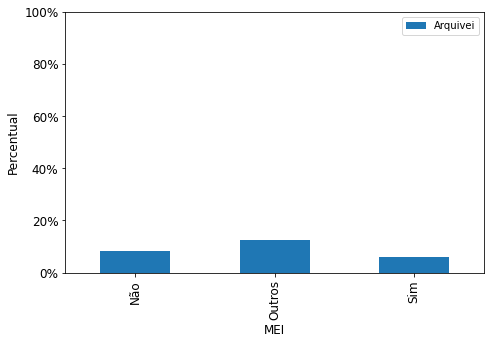
\includegraphics[scale=0.45]{images/base-de-dados-5.1-presenca-por-mei.png}
        \caption{Percentual das empresas presente na base de dados categorizadas pela opção por MEI}
        \label{fig:base-de-dados:descritiva-5.1-presenca-por-mei}
    \end{subfigure} ~ \quad
    \begin{subfigure}[b]{0.45\textwidth}
        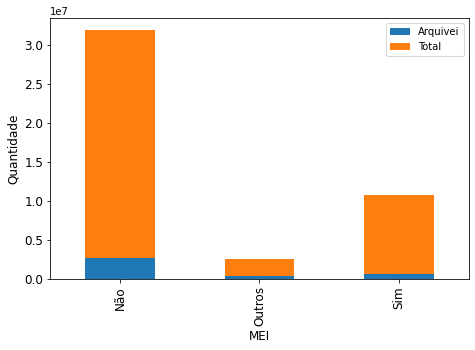
\includegraphics[scale=0.45]{images/base-de-dados-5.2-qtde-por-mei.png}
        \caption{Quantidade de empresas categorizadas pela opção por MEI presente na base de dados relativa ao total}
        \label{fig:base-de-dados:descritiva-5.2-qtde-por-mei}
    \end{subfigure}
    \fdadospesquisa
\end{figure}

\begin{table}[htb]
\centering
\caption{Métricas sobre o percentual das empresas presentes na base de dados pela opção pelo MEI}
\label{tab:participacao-por-mei}
\begin{tabular}{lr}
\toprule
Opção pelo MEI & Participação \\
\midrule
Não      &    10.20\% \\
Outros   &     7.03\% \\
Sim      &     5.98\% \\
\bottomrule
\end{tabular}
\fdadospesquisa
\end{table}

A Lei nº 123/2006 \cite{lei:123:lei-estatuto-mei-e-epp} institui o Simples Nacional, um regime tributário que facilita o recolhimentos de impostos para MEIs e EPPs. A base de dados abertos da Receita Federal também possui a informação da opção ou não pelo regime Simples Nacional. As empresas podem solicitar a exclusão do regime Simples Nacional mediante apresentação de ofício, ou em alguns casos previstos na lei onde a empresa deixa de cumprir alguns requisitos ou obrigações, nestes casos a empresa consta na base de dados como Excluído.

As Figuras~\ref{fig:base-de-dados:descritiva-6-presenca-por-simples-nacional} e~\ref{fig:base-de-dados:descritiva-6.2-qtde-por-simples-nacional}, detalhados na Tabela~\ref{tab:participacao-por-simples-nacional}, mostram a relação entre os dados presentes na base de dados em relação aos totais coletados da Receita Federal. É possível verificar que na base de dados é mais comum a presença de empresas optantes pelo regime Simples Nacional, e assim como em relação à opção ou não pelo MEI isso pode ser um fator de resiliência ou não à crises.

\begin{figure}[htb]
    \centering
    \caption{Participação por região das empresas presentes na base de dados}
    \label{fig:base-de-dados:descritiva-6-presenca-por-simples-nacional}
    \begin{subfigure}[b]{0.45\textwidth} 
        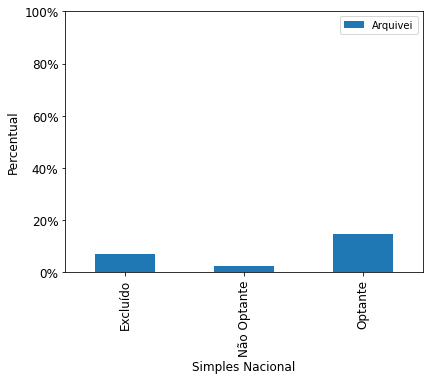
\includegraphics[scale=0.45]{images/base-de-dados-6.1-presenca-por-simples-nacional.png}
        \caption{Percentual das empresas presente na base de dados categorizadas pela opção pelo Simples Nacional}
        \label{fig:base-de-dados:descritiva-6.1-presenca-por-simples-nacional}
    \end{subfigure} ~ \quad
    \begin{subfigure}[b]{0.45\textwidth}
        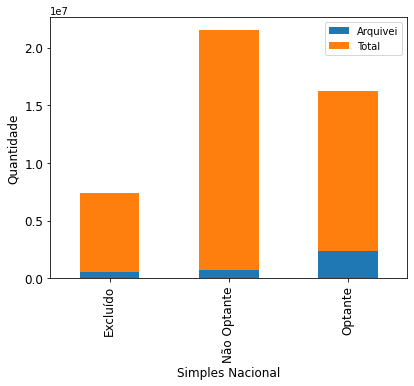
\includegraphics[scale=0.45]{images/base-de-dados-6.2-qtde-por-simples-nacional.png}
        \caption{Quantidade de empresas categorizadas pela opção pelo Simples Nacional presente na base de dados relativa ao total}
        \label{fig:base-de-dados:descritiva-6.2-qtde-por-simples-nacional}
    \end{subfigure}
    \fdadospesquisa
\end{figure}

\begin{table}[htb]
\centering
\caption{Métricas sobre o percentual das empresas presentes na base de dados pela Opção pelo Simples Nacional}
\label{tab:participacao-por-simples-nacional}
\begin{tabular}{lr}
\toprule
Opção pelo Simples Nacional & Participação \\
\midrule
Excluído     &    0.0693 \\
Não Optante  &    0.0229 \\
Optante      &    0.1450 \\
\bottomrule
\end{tabular}
\fdadospesquisa
\end{table}

\subsection{Abrangência setorial}

Nesta Seção, será feita a análise comparativa dos dados presentes na base de dados de documentos fiscais em relação aos dados abertos descritos na Seção~\ref{section:dados-abertos-receita} visando descrever a participação em relação aos setores econômicos da economia brasileira.

Como citado no Capítulo~\ref{chapter:documenos-fiscais}, através dos protocolos do ENAT foi feito o compromisso para a unificação do Cadastro Nacional de Atividades Econômicas (CNAE). Esse cadastro foi implementado então pela Resolução IBGE/CONCLA \sigla*{CONCLA}{Comissão Nacional de Classificação} nº 01 de 04 de setembro de 2006 \cite{resolucao-concla:01:cnae} e Resolução IBGE/CONCLA nº nº 02, de 15 de dezembro de 2006 \cite{resolucao-concla:02:cnae}. Como descrito no Art. 1º da Resolução nº 01, essa classificação é hierárquica:

\begin{citacao}
O PRESIDENTE DA COMISSÃO NACIONAL DE CLASSIFICAÇÃO –
CONCLA, no uso de suas atribuições, resolve:

Art. 1 o Aprovar e divulgar a estrutura completa da Classificação Nacional de Atividades Econômicas – CNAE – versão 2.0, organizada em cinco níveis hierárquicos: seções, divisões, grupos, classes e subclasses, sendo o detalhamento das subclasses destinado ao uso da Administração Pública Brasileira.

(...)
\end{citacao}

O anexo de tal resolução contém uma tabela com o detalhamento dessa classificação, posteriormente retificada.

As empresas informam o código de sua CNAE Fiscal no momento da sua inscrição no Cadastro Nacional de Pessoas Jurídicas, e este dado fica disponível para consulta pública através de sua base de dados aberta. São informadas também os códigos de suas CNAEs secundários referentes a atividades secundárias das empresas, estes não foram utilizados nesta análise.

O Quadro~\ref{quadro:denominacao-secao-cnae} descreve a que se refere cada seção segundo o IBGE/CONCLA.

\begin{quadro}[htb]
\caption{Denominação das Seções de CNAE}
\label{quadro:denominacao-secao-cnae}
\centering
\begin{tabularx}{\textwidth}{|l|l|X|}        \hline
\textbf{Seção} & \textbf{Faixa de Divisões} & \textbf{Denominação} \\ \hline
A & 01 a 03 & Agricultura, pecuária, produção florestal, pesca e aquicultura \\ \hline
B & 05 a 09 & Indústrias extrativas \\ \hline
C & 10 a 33 & Indústrias de transformação \\ \hline
D & 35      & Eletricidade e gás \\ \hline
E & 36 a 39 & Água, esgoto, atividades de gestão de resíduos e descontaminação \\ \hline
F & 41 a 43 & Construção \\ \hline
G & 45 a 47 & Comércio; Reparação de veículos automotores e motocicletas \\ \hline
H & 49 a 53 & Transporte, armazenagem e correio \\ \hline
I & 55 a 56 & Alojamento e alimentação \\ \hline
J & 58 a 63 & Informação e comunicação \\ \hline
K & 64 a 66 & Atividades financeiras, de seguros e serviços relacionados \\ \hline
L & 68      & Atividades imobiliárias \\ \hline
M & 69 a 75 & Atividades profissionais, científicas e técnicas \\ \hline
N & 77 a 82 & Atividades administrativas e serviços complementares \\ \hline
O & 84      & Administração pública, defesa e seguridade social \\ \hline
P & 85      & Educação \\ \hline
Q & 86 a 88 & Saúde humana e serviços sociais \\ \hline
R & 90 a 93 & Artes, cultura e serviços sociais \\ \hline
S & 94 a 96 & Outras atividades de serviços \\ \hline
T & 97      & Serviços Domésticos \\ \hline
U & 99      & Organismos internacionais e outras instituições extraterritoriais \\ \hline
\end{tabularx}
\end{quadro}

As Figuras~\ref{fig:base-de-dados:descritiva-7.1-presenca-por-secao} e \ref{fig:base-de-dados:descritiva-7.2-qtde-por-secao} descrevem a participação percentual por seção econômica e suas quantidades em relação aos totais. A Tabela~\ref{tab:participacao-por-secao} descreve a participação percentual em detalhes.

\begin{figure}[htb]
    \centering
    \caption{Participação por seção do CNAE das empresas presentes na base de dados}
    \label{fig:base-de-dados:descritiva-7-presenca-por-secao}
    \begin{subfigure}[b]{1.0\textwidth} 
        \centering
        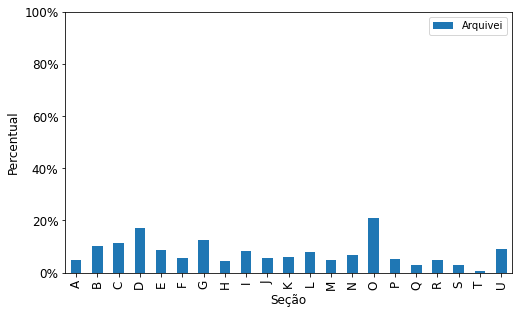
\includegraphics[scale=0.7]{images/base-de-dados-7.1-presenca-por-secao.png}
        \caption{Percentual das empresas presente na base de dados categorizadas pela seção do CNAE}
        \label{fig:base-de-dados:descritiva-7.1-presenca-por-secao}
    \end{subfigure} ~ \\
    \begin{subfigure}[b]{1.0\textwidth}
        \centering
        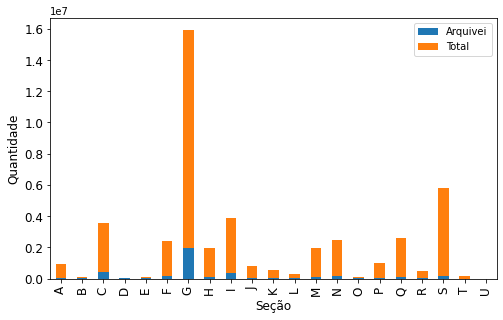
\includegraphics[scale=0.7]{images/base-de-dados-7.2-qtde-por-secao.png}
        \caption{Quantidade de empresas categorizadas seção do CNAE presente na base de dados relativa ao total}
        \label{fig:base-de-dados:descritiva-7.2-qtde-por-secao}
    \end{subfigure}
    \fdadospesquisa
\end{figure}

\begin{table}[htb]
\centering
\caption{Métricas sobre o percentual das empresas presentes na base de dados por Seção do CNAE}
\label{tab:participacao-por-secao}
\begin{subtable}[h]{0.45\textwidth}
    \centering
    \begin{tabular}{l|r}
        \toprule
        Seção & Participação \\
        \midrule
        A     &     4.74\% \\
        B     &    10.31\% \\
        C     &    11.30\% \\
        D     &    17.17\% \\
        E     &     8.69\% \\
        F     &     5.66\% \\
        G     &    12.34\% \\
        H     &     4.36\% \\
        I     &     8.40\% \\
        J     &     5.41\% \\
        K     &     5.91\% \\
        \bottomrule
    \end{tabular}
\end{subtable}
\begin{subtable}[h]{0.45\textwidth}
    \centering
    \begin{tabular}{l|r}
        \toprule
        Seção & Participação \\
        \midrule
        L     &     7.87\% \\
        M     &     4.71\% \\
        N     &     6.66\% \\
        O     &    20.72\% \\
        P     &     5.22\% \\
        Q     &     3.01\% \\
        R     &     4.75\% \\
        S     &     2.82\% \\
        T     &     0.71\% \\
        U     &     9.07\% \\
        \bottomrule
    \end{tabular}
\end{subtable}
\fdadospesquisa
\end{table}

Através destes dados é possível notar que existe uma participação significativa em praticamente todas as seções, com exceção da seção T, de serviços domésticos. Os dados também possuem razoável viés para alguns setores que possuem altos percentuais, particularmente D, G, e O, em oposição aos outros. A quantidade de empresas de cada seção também varia significativamente, particularmente a seção G que possui um número bastante alto de empresas, o que não necessariamente implica maior quantidade de documentos fiscais ou valor transacionado, análise que será feita posteriormente.

A Figura~\ref{fig:base-de-dados:descritiva-9.1-presenca-por-cnae} ilustra a participação percentual por CNAE, e a Tabela~\ref{tab:participacao-por-cnae} nos dá algumas métricas acerca da participação por CNAE. Dos 1342 CNAEs existentes na base de dados de comparação, 1327 são citados na base de dados de documentos fsicais (98.88\%), com uma média de cerca de 15\% de participação e desvio padrão de cerca de 12\%.

É possível observar então que que há uma grande abrangência setorial, uma vez que a base de dados possui exemples da grande maioria das seções, mas o histograma mostra que existe uma grande quantidade de CNAEs com baixo percentual de participação.

\begin{figure}[htb]
	\centering
    \caption{Histograma do percentual das empresas de cada CNAE presente na base de dados}
    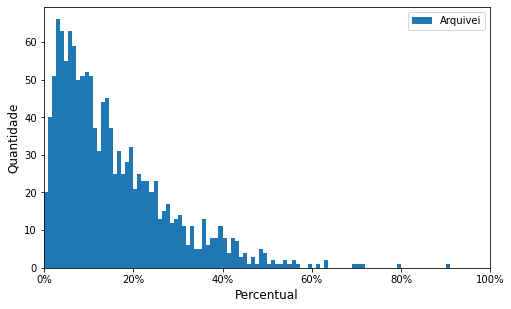
\includegraphics[scale=0.7]{images/base-de-dados-9.1-presenca-por-cnae.png}
    \label{fig:base-de-dados:descritiva-9.1-presenca-por-cnae}
    \fdadospesquisa
\end{figure}

\begin{table}[htb]
\centering
\caption{Métricas sobre o percentual das empresas presentes na base de dados por  CNAE}
\label{tab:participacao-por-cnae}
\begin{tabular}{lr}
\toprule
Métrica & Valor \\
\midrule
Média         &   15.371\% \\
Desvio Padrão &   12.452\% \\
Mínimo        &    0.004\% \\
25º percentil &    5.984\% \\
50º percentil &   12.056\% \\
75º percentil &   21.570\% \\
Máximo        &   90.909\% \\
\bottomrule
\end{tabular}
\fdadospesquisa
\end{table}
